% !TeX root = ../libro.tex
% !TeX encoding = utf8

\chapter{Análisis y diseño}

En este capítulo se especificará toda aquella información referente a la estructura del programa y los requisitos del mismo, aunque está mayormente enfocado a la definición de los algoritmos desarrollados.

\section{Especificación de requisitos}

	\subsection*{Requisitos funcionales}
	\begin{enumerate}
		\item Se podrán visualizar varias parametrizaciones a la vez, donde cada una representará una carta de una superficie específica, con el objetivo de representar homotopías e isotopías entre superficies.
		\begin{enumerate}
			\item El sistema debe permitir visualizar cualquier parametrización que se le indique, siempre que cumpla con la estructura del lenguaje definido.
			\item Cada parametrización podrá admitir parámetros de ``tiempo'', para así modificar la porción de superficie que representa y así poder visualizar homotopías e isotopías.
		\end{enumerate}
		
		\item El programa contará con una interfaz clara, sencilla y completa.
		\begin{enumerate}
			\item El usuario tendrá la posibilidad de indicar manualmente los parámetros adicionales de las cartas $(t_i)$. Además se incluirá la opción de que cada $t_i$ se mueva de forma automática, para así generar animaciones fluidas.
			
			\item El usuario podrá indicar ciertos parámetros del cálculo de la malla de la superficie, como:
			\begin{enumerate}
				\item El tamaño de la malla inicial con la que se visualizará cada carta de la superficie.
				\item La precisión con la que se quiere representar la superficie actual.
			\end{enumerate}
				
			\item El usuario podrá indicar si quiere visualizar ciertos atributos de la superficie, como:
			\begin{enumerate}
				\item La curvatura de Gauss, asignando un color para la curvatura negativa y otro para la positiva, dependiendo de un parámetro de escala para resaltar las zonas.
				\item El área diferencial de la parametrización, junto con un umbral y un factor de escala que se podrán modificar.
				\item Se podrán visualizar los vectores tangente, bitangente y normal de cada vértice generado.
			\end{enumerate}
			
			\item El usuario tendrá la posibilidad de modificar los valores referentes a la iluminación.
			\begin{enumerate}
				\item Los coeficientes del modelo de iluminación Phong.
				\item El color del fondo de la escena y el color base del objeto visualizado.
			\end{enumerate}
		\end{enumerate}
			
		\item El programa no renderizará nuevos frames si no se requieren nuevos cálculos, es decir, si no se detectan cambios en la entrada y la escena está estática.
	\end{enumerate}

	\subsection*{Requisitos no funcionales}
	\begin{enumerate}
		\item El programa debe renderizar las superficies con un tiempo de respuesta bajo, pensando en dispositivos con una GPU común, como por ejemplo una gráfica integrada.
		\begin{enumerate}
			\item El programa adaptará su rendimiento según el estado del propio programa.
		\end{enumerate}
	\end{enumerate}

\section{Diagramas}
En esta sección se ilustran ciertos diagramas que facilitan el entendimiento del programa. Los siguientes diagramas están relacionados con la acción ``compilar'', que es la que implica mayor comunicación entre entidades, donde cabe destacar que ``lastParam.in'' es donde se encuentra la parametrización de la superficie en texto, ``error.log'' es donde se almacena la salida de error, ``temp'' donde se indican el nº de cartas a visualizar (y el nº máximo de parámetros) y ``functions.s'' el código GLSL para los shaders.\\
\begin{figure}[h]
  	\centering
  	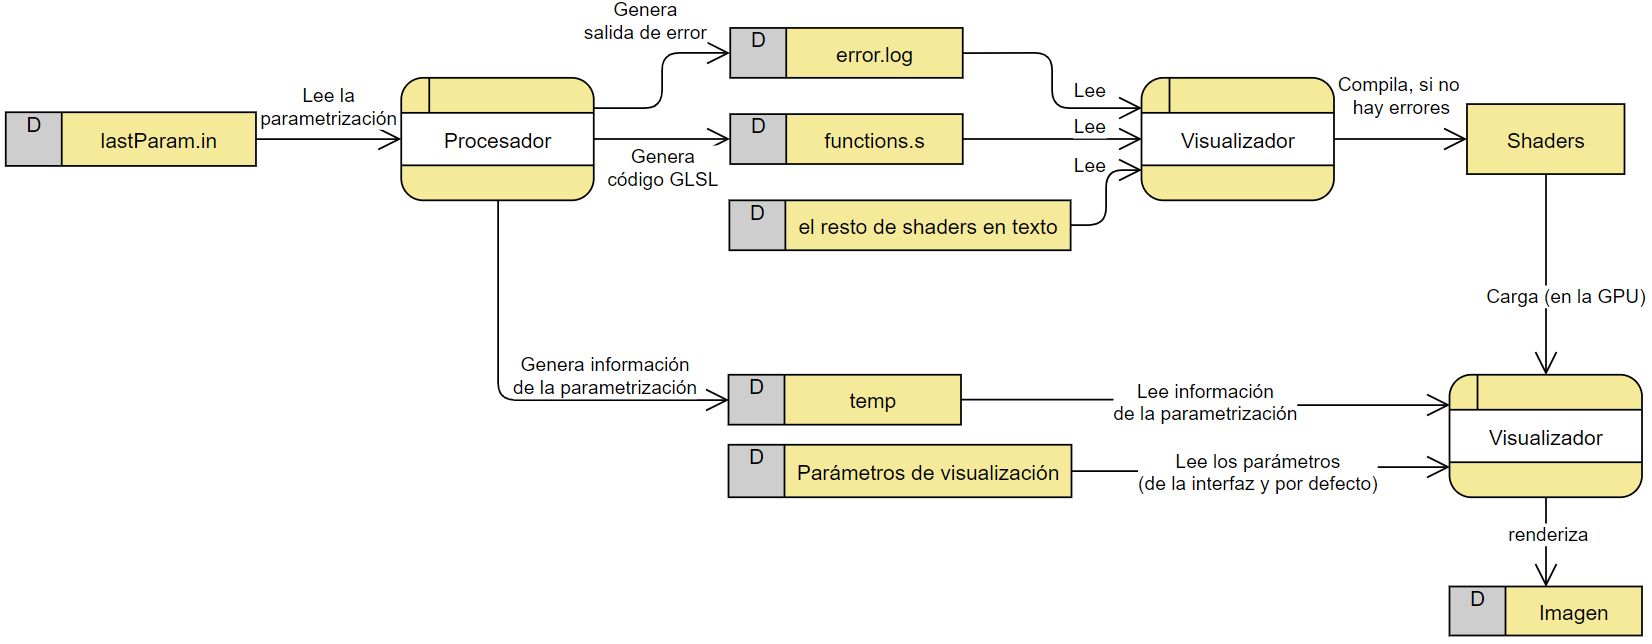
\includegraphics[width=1\textwidth]{diagrama_dfd}
  	\caption{Diagrama de flujo de datos tras ejecutar la acción ``compilar''.}
  	\label{fig:diagrama_dfd}
\end{figure}
\newpage
\begin{figure}[h]
  	\centering
  	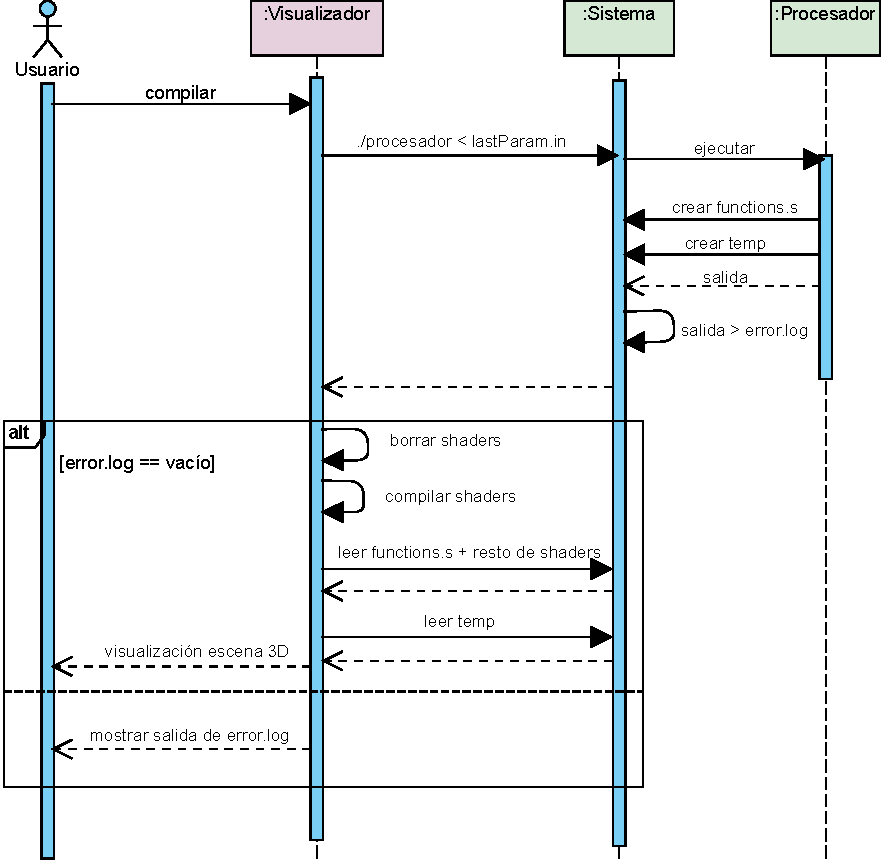
\includegraphics[width=0.8\textwidth]{diagrama_interaccion}
  	\caption{Diagrama de interacción de la acción ``compilar''.}
  	\label{fig:diagrama_interaccion}
\end{figure}
\newpage
Además se muestran los bocetos iniciales de la interfaz de usuario, incluyendo únicamente las agrupaciones de elementos, ya que la distribución de botones y otras entidades se desconocía a priori (no se sabía cuáles serían necesarios ni en qué forma, hasta un punto más avanzado del proyecto).\\
\begin{figure}[h]
  	\centering
  	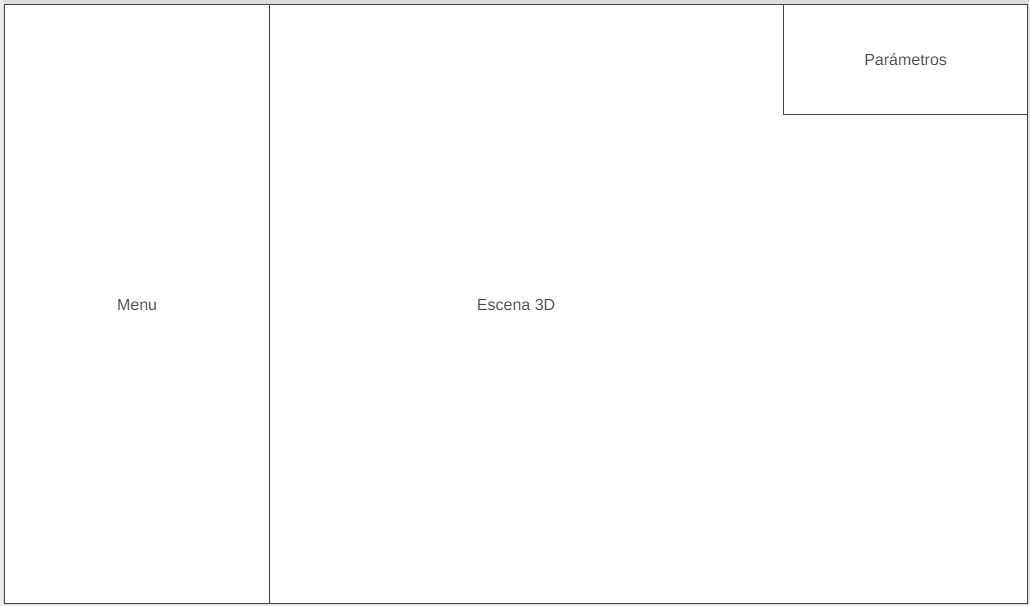
\includegraphics[width=0.8\textwidth]{boceto1}
  	\caption{Boceto de la interfaz con los elementos principales.}
  	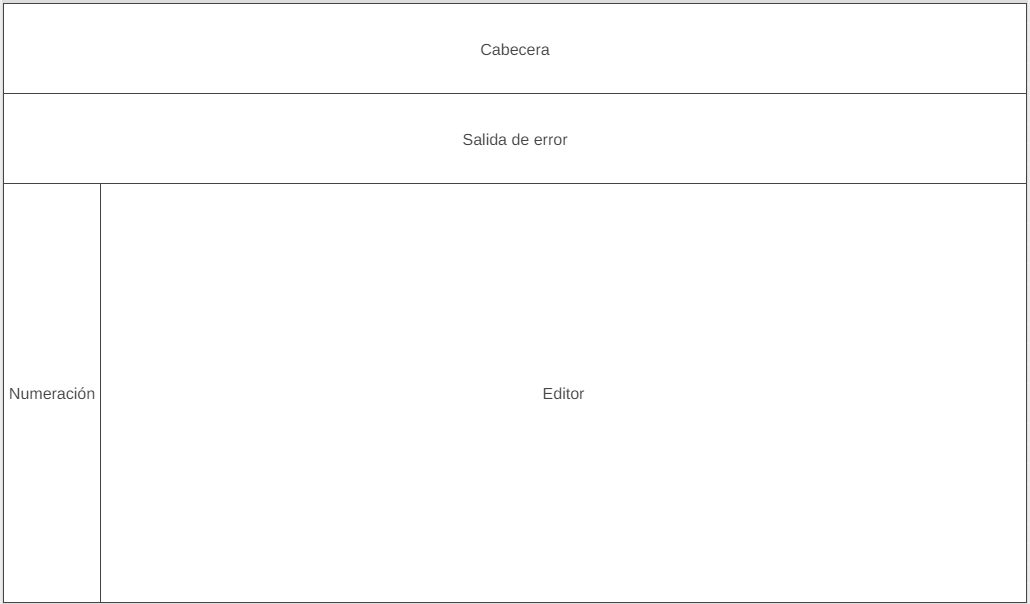
\includegraphics[width=0.8\textwidth]{boceto2}
  	\caption{Boceto de la ventana de edición de código.}
  	\label{fig:bocetos_interfaz}
\end{figure}
\\Cabe destacar que al final la interfaz en su totalidad está compuesta por ventanas móviles y contraíbles, aportando mayor flexibilidad y comodidad al usuario, sobretodo si quiere ver la escena en pantalla completa.

\section{Principales estructuras de datos}

La estructura de datos más interesante y que destaca fuera de lo normal es la de nodo de expresión (nodo), utilizada en el programa ``procesador'' para representar los árboles de expresión. Es un ``struct'' con los siguientes componentes:
\begin{itemize}
	\item char *lex; representa el lexema del nodo: el nombre de la función a la que llama, el lexema del operador, el nombre de la variable o la cte.
	\item struct nodo *children[10]; los hijos del nodo (10 máximo, pero ampliable si fuese necesario).
	\item int nchild; el nº de descendientes que realmente tiene el nodo.
	\item tipoNodo tipo; indica el tipo de nodo de expresión: cte, variable, operador, función, índice, paréntesis o condicional (if).
	\item tipoNodoArray subTipo, indica el tipo de dato que maneja el nodo, es decir, si utiliza escalares, vectores o matrices, junto con sus respectivas dimensiones (son siempre cuadradas, por similitud al lenguaje GLSL).
\end{itemize}

\section{Principales desarrollos algorítmicos}

Aunque en el capítulo $5$ de esta segunda parte se ha descrito con detalle el estudio del teselado, que está directamente ligado con el algoritmo de teselación, en esta sección se hablará del resto de desarrollos algorítmicos, los cuales están relacionados con el procesador del lenguaje (programa ``Procesador'').

\subsection*{Generación de árboles de expresión}
Se generan de forma natural al realizar el análisis sintáctico con el procesador. Cuando se reduce la expresión por una regla, en dicha regla se crea un nodo de expresión nuevo y se le asigna a la variable a la que se reduce, con los hijos y características correspondientes.

\subsection*{Obtener el árbol de la derivada parcial de una expresión}
El software implementado es capaz de hacer derivación simbólica, útil para la generación automática de funciones típicas de una superficie, como la normal o la curvatura de Gauss.\\
\\Dado un árbol de expresión y una variable, el cálculo del árbol de la derivada parcial respecto de dicha variable se realiza de manera recursiva, aplicando las reglas usuales de derivación. \\
\\El caso más complejo, que cabe destacar, es cuando se trata de una llamada a otra función ya definida por el usuario, cuyos parámetros contienen la variable a derivar. Entonces se aplica la regla de la cadena para derivadas parciales, es decir:
$$\frac{\partial}{\partial u}(f(exp_1, ..., exp_n)) = \sum_{i=1}^{n} \frac{\partial (exp_i)}{\partial u} \frac{\partial f}{\partial x_i}(exp_1, ..., exp_n))$$
Pero es necesario definir la función $\frac{\partial f}{\partial x_i}$ $\forall i$, así que se comprobaría si existen ya dichas funciones y en caso negativo se definirán (se deriva su árbol de expresión asociado y se escribe en una función con nombre $fPx_i$).

\subsection*{Simplificación de las expresiones}
La simplificación de una expresión consiste en quitar paréntesis redundantes y eliminar aquellas operaciones evitables, como sumar $0$ o multiplicar por $1$. Esto mejora la legibilidad del código de salida.\\
\\Dado un árbol de expresión, su simplificación se realiza de forma recursiva. Si denominamos $simplificar(n)$ a la función que devuelve el árbol de expresión simplificado, con $n$ el nodo raíz, entonces el algoritmo es el siguiente:
\begin{enumerate}
	\item Si $n$ tiene hijos $n_i$, ejecutar $simplificar(n_i)$.
	\item Si $n$ es un nodo de paréntesis y su hijo no es un nodo de operación, sustituye $n$ por su propio hijo (quita los paréntesis).
	\item Si $n$ es un nodo de operador y algún hijo es $0$ o $1$, se dice que puede ser simplificable:
	\begin{itemize}
		\item Si el operador es unario, entonces:
		\begin{itemize}
			\item Si el nodo hijo es $0$ y el operador es $-$, se sustituye el nodo padre por el nodo hijo (quitar el signo).
			\item Si el operador es !, entonces se sustituye el nodo padre por el contrario (aplica la negación).
		\end{itemize}
		\item Si el operador es binario, entonces (entendemos $i,j \in \{1,2\}$, $i \neq j$):
		\begin{itemize}
			\item Si el nodo hijo $n_i$ es $0$ y el operador es $+$, se sustituye el nodo padre por el nodo hijo $n_j$.
			\item Si el nodo hijo $n_2$ es $0$ y el operador es $-$, se sustituye el nodo padre por el nodo hijo $n_1$.
			\item Si el nodo hijo $n_1$ es $0$ y el operador es $-$, se elimina el nodo hijo $n_2$ (queda como operador unario).
			\item Si el nodo hijo $n_i$ es $0$ y el operador es $*$, se sustituye el nodo padre por el nodo cte $0$.
			\item Si el nodo hijo $n_i$ es $1$ y el operador es $*$, se sustituye el nodo padre por el nodo hijo $n_j$.
			\item Si el nodo hijo $n_1$ es $0$ y el operador es $/$, se sustituye el nodo padre por el nodo cte $0$.
			\item Si el nodo hijo $n_2$ es $1$ y el operador es $/$, se sustituye el nodo padre por el nodo hijo $n_1$.
		\end{itemize}
	\end{itemize}
\end{enumerate}

\newpage
A continuación se ilustra el árbol asociado a la expresión  $u^\wedge 2 * v + 1$, junto con el árbol de su derivada parcial respecto de $u$ y su posterior simplificación (sólo teniendo en cuenta los operadores -, +, * y /). La potencia con exponente $1$ no se simplifica puesto que no se ha implementado (principalmente porque tras derivar siempre se escribe como un flotante), aunque en un futuro se podría mejorar, junto con técnicas de simplificación más complejas, para así reducir el tiempo de compilación de los shaders y realizar menos cálculos costosos.

\begin{figure}[h]
		\begin{minipage}{0.35\textwidth}
  			\centering
		  	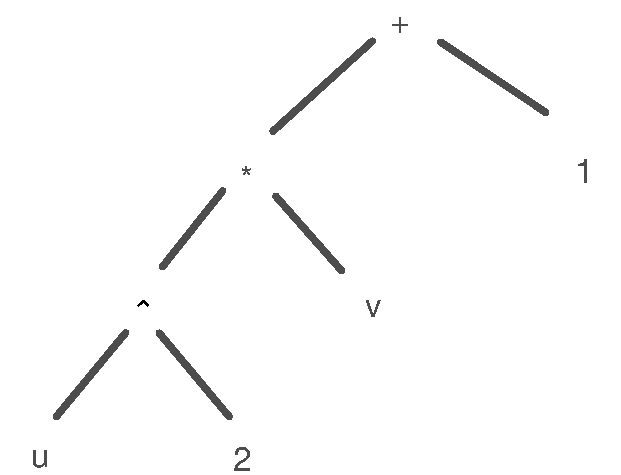
\includegraphics[width=1\textwidth]{expresion}
		\end{minipage}\hfill
		\begin{minipage}{0.4\textwidth}
  			\centering
		  	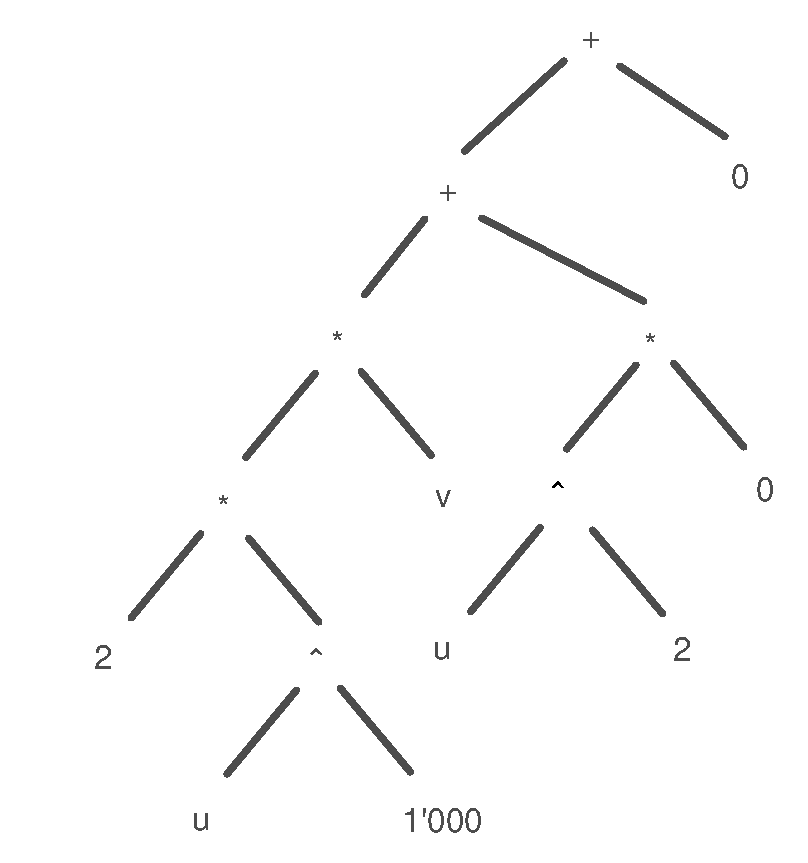
\includegraphics[width=1\textwidth]{partial_expresion}
		\end{minipage}\hfill
		\begin{minipage}{0.23\textwidth}
  			\centering
		  	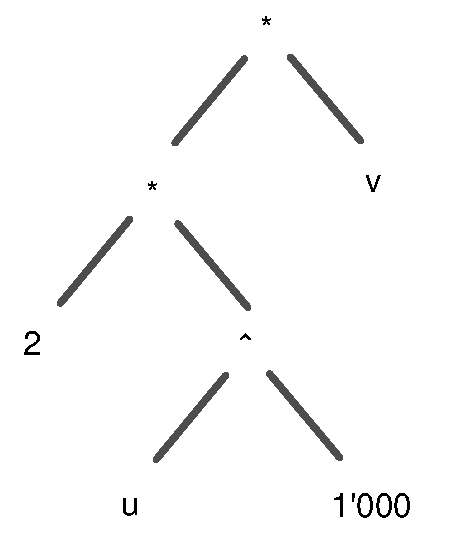
\includegraphics[width=1\textwidth]{simplified}
		\end{minipage}\hfill
	\caption{Árbol de la expresión, su parcial respecto $u$ y el mismo pero simplificado.}
  	\label{fig:arbol_expresion}
\end{figure}

\endinput
%------------------------------------------------------------------------------------
% FIN DEL CAPÍTULO. 
%------------------------------------------------------------------------------------
